\begin{figure*}[!t]
    \centering
    % Kolom kiri (gambar 1 di atas, gambar 2 di bawah)
    \begin{minipage}{0.48\textwidth}
        \centering
        % Gambar pertama dengan highlight
        \begin{tikzpicture}
            \node[anchor=south west,inner sep=0] (img1)
                {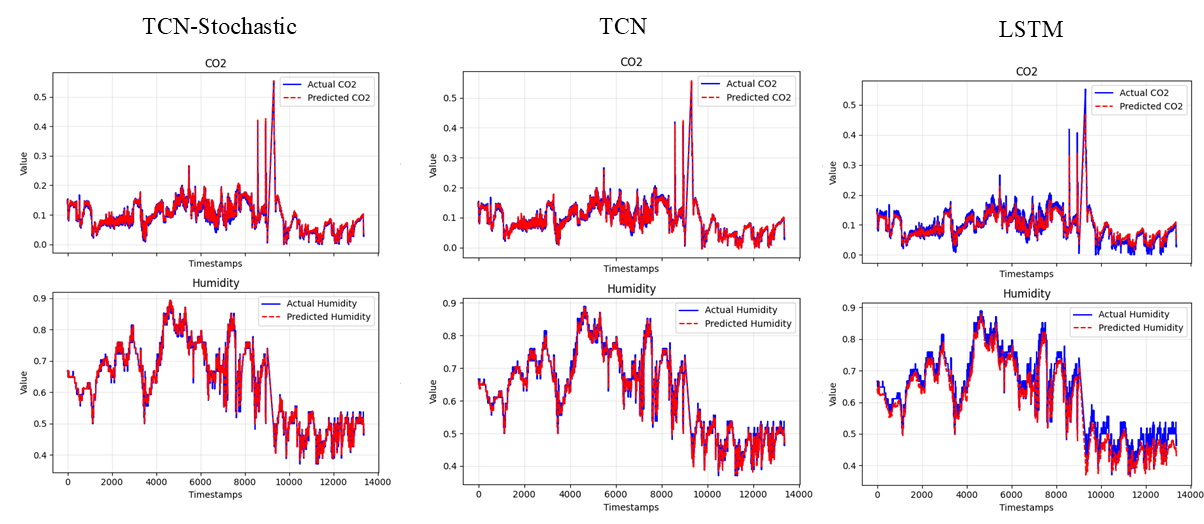
\includegraphics[width=\textwidth]{images/tcns-tcn-lstm.PNG}};
            % Highlight rectangle
            \begin{scope}[x={(img1.south east)},y={(img1.north west)}]
                \draw[blue, thick, dashed] 
                    (0.01,0.01) rectangle (0.33,0.99);
            \end{scope}
        \end{tikzpicture}

        % Gambar kedua (tanpa highlight)
        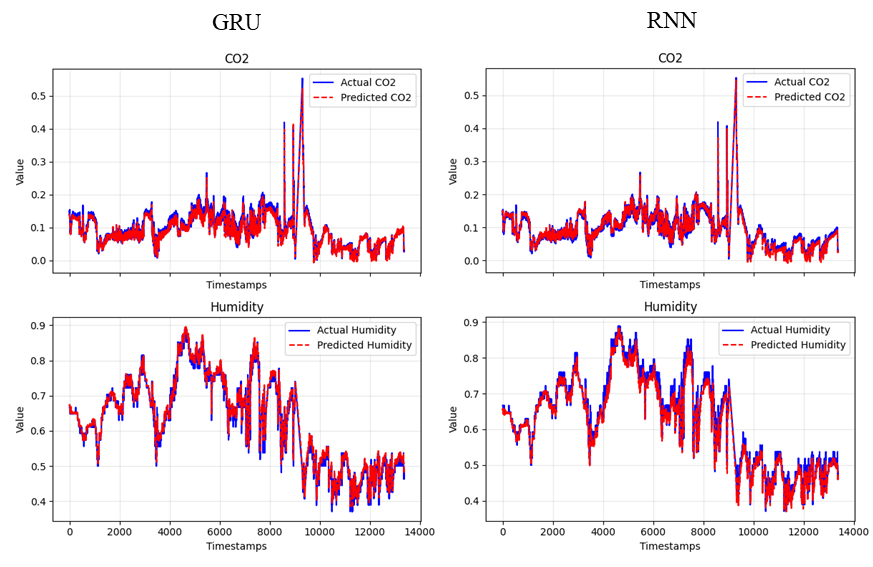
\includegraphics[width=\textwidth]{images/gru-rnn.PNG}
        \caption*{(a) A comparative analysis between the TCN-Stochastic and baseline models was conducted using test data for $CO_2$ and humidity. The top row shows TCN‑Stochastic, TCN, and LSTM, while the bottom row presents GRU and RNN in sequence from left to right respectively.} 
    \end{minipage}
    \hfill
    % Kolom kanan (gambar 3 di atas, gambar 4 di bawah)
    \begin{minipage}{0.48\textwidth}
        \centering
        % Gambar pertama dengan highlight
        \begin{tikzpicture}
            \node[anchor=south west,inner sep=0] (img1)
                {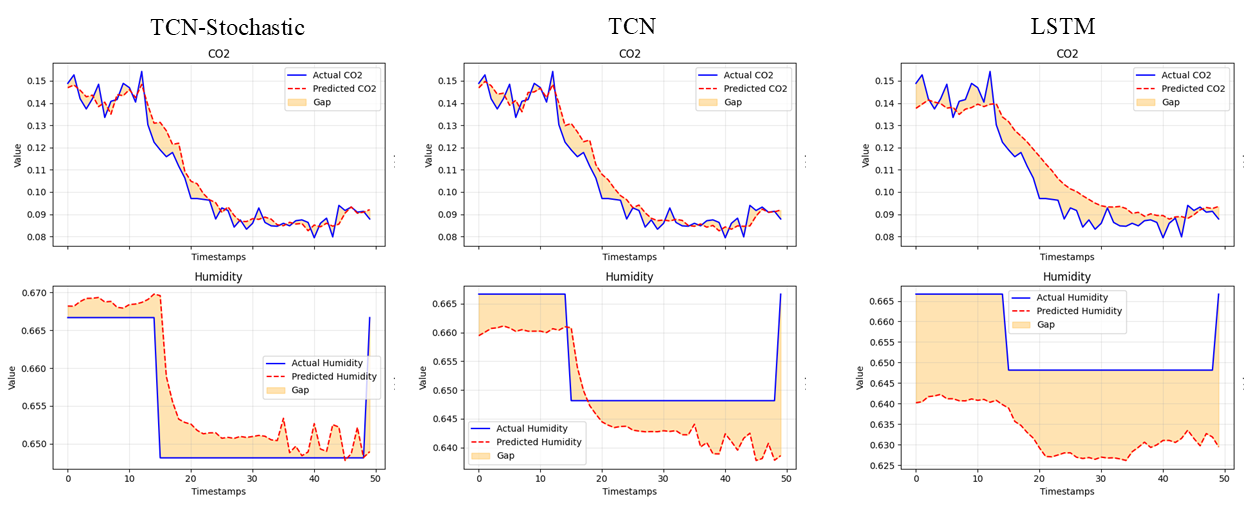
\includegraphics[width=\textwidth]{images/60 steps - tcns-tcn-lstm.PNG}};
            % Highlight rectangle
            \begin{scope}[x={(img1.south east)},y={(img1.north west)}]
                \draw[blue, thick, dashed] 
                    (0.01,0.01) rectangle (0.33,0.99);
            \end{scope}
        \end{tikzpicture}
        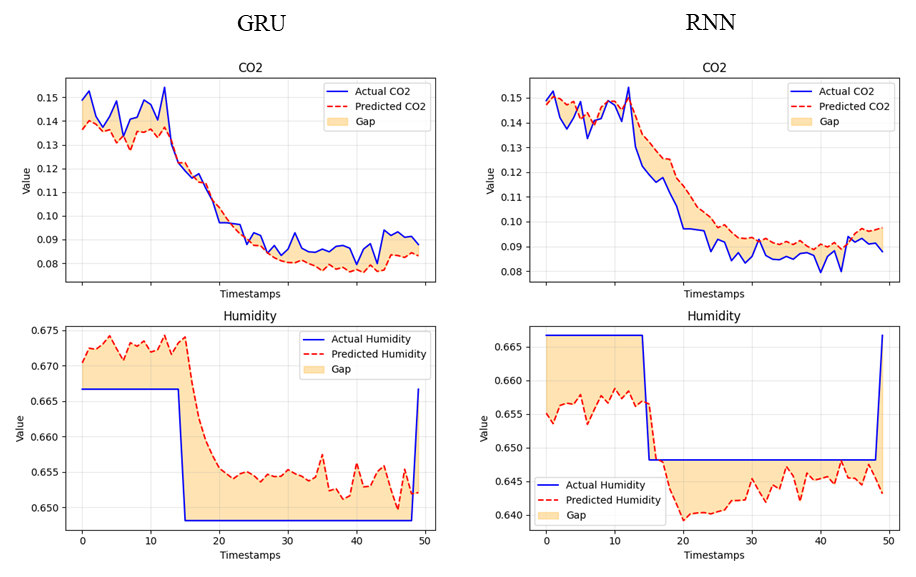
\includegraphics[width=\textwidth]{images/60 steps - gru - rnn.PNG}
        \caption*{(b) A comparative analysis of predicted versus actual values for $CO_2$ and humidity over 60 timesteps is presented. The top row shows TCN‑Stochastic, TCN, and LSTM models, while the bottom row displays GRU and RNN in sequence from left to right respectively.}
    \end{minipage}

    \caption{The Comparison analysis of model prediction results in displaying actual vs predicted values of testing dataset.}
    \label{fig:feature-timestep}
\end{figure*}